\documentclass[a4paper,french,oneside,10pt]{book}
\usepackage[utf8]{inputenc}
\usepackage[french]{babel}
\usepackage[colorlinks=true]{hyperref}
\hypersetup{urlcolor=blue,linkcolor=red,colorlinks=false} 
\usepackage{fancyhdr}
\usepackage{enumerate}
\usepackage{graphicx}
\usepackage[french]{minitoc}
\usepackage{multirow}
\usepackage{placeins}
\usepackage{listings}
\usepackage{color}
\usepackage{float}
\usepackage{tabularx}
\usepackage{amsmath}
\usepackage{amssymb}
\usepackage[french]{varioref}
%\usepackage[bookmarks=true]{hyperref}
\usepackage{lscape}
\usepackage[xindy,toc,acronym]{glossaries}
\usepackage{setspace}
\usepackage{algorithm,algorithmic}
\usepackage{xparse}

\usepackage{tikz}
\usetikzlibrary{trees}
\usetikzlibrary{arrows,shapes}

\usepackage[normalsize]{subfigure}
\usepackage{verbatim}

\tikzstyle{vertex}=[circle,fill=black!25,minimum size=20pt,inner sep=0pt]
\tikzstyle{edge} = [draw,thick,-]
\tikzstyle{tree edge} = [draw, thick,->,red!75]
\tikzstyle{queue edge} = [draw,thick,->,blue!50]
\tikzstyle{cross} = [path picture={ \draw[black](path picture bounding box.south east) -- (path picture bounding box.north west) (path picture bounding box.south west) -- (path picture bounding box.north east);}]
\pgfdeclarelayer{background}
\pgfsetlayers{background,main}

\NewDocumentEnvironment{coolquote}{O{}}{%
\vspace{0.2cm}
\itshape
\raisebox{-.05\linewidth}{
\includegraphics[width=.1\linewidth]{guillemet}}%
\hspace{0.1cm}
\begin{minipage}[t]{.85\linewidth}
}{
\end{minipage}
\begin{minipage}[t]{\linewidth}
\vspace{0.2cm}
\hfill\normalfont\scriptsize #1
\end{minipage}
\vspace{0.2cm}
}

% Romain
\newcommand{\cRM}[1]{\MakeUppercase{\romannumeral #1}}  % Capital
\newcommand{\cRm}[1]{\textsc{\romannumeral #1}} % Petit majuscule
\newcommand{\crm}[1]{\romannumeral #1}
% Siècle %
\newcommand{\siecle}[1]{\cRM{#1}\textsuperscript{e}~siècle}

\hypersetup{pdfborder={0 0 0}}
\pagestyle{fancy}
\setlength{\parskip}{1.5ex plus .4ex minus .4ex}
\renewcommand{\labelitemi}{\textbullet}
\renewcommand{\chaptermark}[1]{\markboth{#1}{}}


\def\doctitle{L'école à l'heure du numérique}

%definition du titre et autres param
\def\titre{\LARGE \doctitle}
\def\sstitre{Épistémologie de l'informatique, décembre 2012}
\def\auteurs{
      Chloé \textsc{Desdouits} \\
      William \textsc{Dyce} \\
      Thibaut \textsc{Marmin} \\
      Clément \textsc{Sipieter}}
      
\def\url{\href{https://github.com/patre/epistemo}{https://github.com/patre/epistemo}}

\newcommand{\method}[1]{\texttt{{#1}}}
\newcommand{\class}[1]{\texttt{{#1}}}
\newcommand{\package}[1]{\textbf{{#1}}}
%\newcommand{\gls}[1]{\newgls{#1}}


\pagestyle{fancy}

\renewcommand{\chaptermark}[1]{\markboth{#1}{}}
\renewcommand{\sectionmark}[1]{\markright{\thesection\ #1}}

\fancyhf{}

\fancyhead[RO,LE]{\thepage}
\fancyhead[LO]{\leftmark}
\fancyhead[RE]{\doctitle}

\fancypagestyle{corps}{ 
\fancyhead[RO,LE]{\thepage}
\fancyhead[LO]{\rightmark}
\fancyhead[RE]{\leftmark}
}

\renewcommand{\footrulewidth}{0pt} % pas de filet en bas
\fancypagestyle{plain}{ % pages de tetes de chapitre
\fancyhead{}
% supprime l’entete
\renewcommand{\headrulewidth}{0pt} % et le filet
}
\newcommand{\clearemptydoublepage}{%
	\newpage{\pagestyle{empty}\cleardoublepage}}


%Modification des marges
%\\oddsidemargin}{-2,5cm}
%\addtolength{\textwidth}{5cm}
%\addtolength{\topmargin}{-2,5cm}
%\addtolength{\textheight}{4cm}

%definition des fonctions de la page de garde
\def\blurb{%
  \begin{tabular}{l p{0.6cm} c p{0.8cm} r}
   \multirow{3}{*}{\vspace{-1.5cm}\hspace{-1cm}
\includegraphics[width=3cm]{./files/um2}} & & & &  \multirow{3}{*}{\vspace{-1.5cm}
\includegraphics[width=2cm]{./files/ufr}} \\
    & & Ministère de l'Éducation Nationale & & \\
    & & Université de Montpellier 2 & & \\ 
    & & Place Eugène Bataillon & & \\ 
    & & 34095 Montpellier Cedex 5 & & \\
    & & & & \\
    & & Épistémologie de l'informatique (FMIN 357)& & \\
    & & Master Informatique 2\ieme année& & \\
    \vspace{0.5cm}
   \end{tabular}
  }
\def\clap#1{\hbox to 0pt{\hss #1\hss}}%
\def\ligne#1{%
  \hbox to \hsize{%
    \vbox{\centering #1}}}%
\def\haut#1#2#3{%
  \hbox to \hsize{%
    \rlap{\vtop{\raggedright #1}}%
    \hss
    \clap{\vtop{\centering #2}}%
    \hss
    \llap{\vtop{\raggedleft #3}}}}%
\def\bas#1#2#3{%
  \hbox to \hsize{%
    \rlap{\vbox{\raggedright #1}}%
    \hss
    \clap{\vbox{\centering #2}}%
    \hss
    \llap{\vbox{\raggedleft #3}}}}%

\makeglossaries
\newglossaryentry{technologie}
{
  name=technologie, 
  plural=technologies,
  description = {Concept relatif à une techniques ou un outil}
}

\newacronym{ticLabel}{TIC}{Technologies de l'Information et de la Communication}

\newacronym{ntic}{NTIC}{Nouvelles Technologies de l'Information et de la Communication}

\newacronym{OLPC}{OLPC}{One Laptop Per Child}

\newacronym{HIW}{HIW}{Hole in the wall}

\newacronym{GCSE}{GCSE}{General Certificate of Secondary Education}

\newacronym{SOLE}{SOLE}{Self Organized Learning Environment}


\begin{document}


\dominitoc

\thispagestyle{empty}
  \vbox to .9\vsize{%
  \vss
  \vbox to 1\vsize{%
    \haut{}{\blurb}{}
    \vfill
    
    \noindent\rule{\linewidth}{.5pt}
    \ligne{\vspace{1.5mm}\titre}
    \noindent\rule{\linewidth}{.5pt}
    \ligne{\normalsize{\textsc{\sstitre}}}
    \vfill
    \ligne{%
      \begin{tabular}{l}
	\vspace{5mm}
      \end{tabular}
      \begin{tabular}{c}
      Travail réalisé par \\\\
       \auteurs
      \end{tabular}
    }
    \ligne{%
    \begin{tabular}{l}          
	\vspace{15mm}
      \end{tabular}
       \texttt{\url}
       }
  \vss
  }
}
\clearemptydoublepage

\chapter*{}
 \vspace*{\stretch{1}}
\begin{center}
\texttt{\LARGE CC BY-SA 3.0}


\includegraphics[scale=0.8]{files/free}

Ce document, réalisé par une équipe de quatre étudiants en Master 2 informatique de l'Université Montpellier 2\footnote{Auteurs :\\ \auteurs}, est mis à disposition selon les termes de la licence Creative Commons Paternité - Partage à l'Identique 3.0 France\footnote{Plus d'informations à l'adresse suivante : \href{http://creativecommons.org/licenses/by-sa/3.0/fr/}{http://creativecommons.org/licenses/by-sa/3.0/fr/}}.
\end{center}
 \vspace*{\stretch{4}}
\clearemptydoublepage

% !TEX encoding = UTF-8 Unicode
% !TEX root = rapport.tex

\chapter{Introduction}\label{intro}





\clearemptydoublepage

% !TEX encoding = UTF-8 Unicode
% !TEX root = rapport.tex

\chapter*{Abstract}\label{abstract}

\begin{coolquote}[Albert Einstein]
\Large Education is what remains when one has forgotten everything one has learnt at school.
\end{coolquote}

\textit{Are memorisation, note-taking and mental calculation really useful abilities that our elders are trying to pass down, or are they simply tools used to sort the intellectual wheat from the chaff? Is education thus a sort of game where one learns skills of little practical use in the "real world"? For even if we consider an individual's intellectual blossoming to the goal of education, learning facts and figures by heart hardly contributes to this.}

\textit{Perhaps it was once much more pertinent, but today there seems to be an ever-greater chasm opening up between the tools that education provides and what society requires. This is especially true of information-technology, which is shaping our world far faster than education can keep up with. But should it "keep up"? In this age of Information, should education change and, if so, how?}

\textit{In the paper we will be discussing the problem of information-technology and education, as well as solutions that have been put forward in recent years.}
\clearemptydoublepage

\tableofcontents
\clearemptydoublepage

% !TEX encoding = UTF-8 Unicode
% !TEX root = rapport.tex

\part{Historique de l'intégration des technologies de l'information \ldots}\label{quoi}

\chapter*{Avant-propos~: Technologies \og{}Informatiques\fg{}?}

\begin{minipage}[H]{0.3\linewidth}
  \begin{figure}[H]
  \centering
  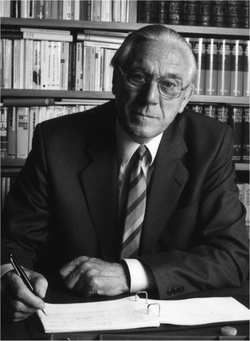
\includegraphics[width=0.8\textwidth]{../resources/illustrations/steinbuch}
  \caption{Karl Steinbuch}
  \end{figure}
\end{minipage}
\begin{minipage}[H]{0.7\linewidth}
Le mot \og{}informatique\fg{} est une concatenation d'\og{}information\fg{} et \og{}automatique\fg{} fait en 1957 par Karl Steinbuch\cite{steinbuch-2005} pour décrire le traitement automatique de l'information.

Depuis le terme a été adopté pour décrire une gamme tellement vaste de sciences, de technologies et de services qu'il a besoin d'être qualifié pour avoir un sens précis.
\vspace{1cm}
\end{minipage}

\begin{coolquote}[Wikipedia\cite{wiki-informatique}]
Les expressions \og{}science informatique\fg{}, \og{}informatique fondamentale\fg{} ou \og{}informatique théorique\fg{} sont utilisées pour désigner sans ambiguïté la science, tandis que \og{}technologies de l'information\fg{} ou \og{}technologies de l'information et de la communication\fg{} désignent le secteur industriel et ses produits.
\end{coolquote}

Ici nous utiliserons \og{}technologies de l'information\fg{} pour décrire toute technique permettant de stoquer, de traiter ou de transférer l'information. Cette définition couvre évidemment les algorithmes, structure données et protocoles de communication, mais aussi les langages naturels, l'écriture, et tout outil de réflexion logico-mathématique\ldots

\chapter{Le langage~: protocole de communication}
Avec l'apparition du langage l'Être humain s'est doté d'un outil capable d'exprimer des informations de plus en plus complexes. Environ 6000 langues sont parlés aujourd'hui et nous n'avons jamais découvert une civilisation démunie d'un langage complexe\cite{linguistics-pinker}. Il est difficile de dater l'appararition du langage. En effet l'homme essaye depuis des milliers d'années de trouver un \og{}proto-language\fg{}, origine de toute autre, sans succès. Dans \og{}L'Enquête\fg{}, l'historien Grecque Hérodote fait référence à une expérience de \og{}privation de langage\fg{} du pharaon Psammétique~I visant à déterminer le langage \og{}par défaut\fg{} de l'Homme\cite{herodote-privation}. 

\begin{minipage}[H]{0.7\linewidth}
De tels expériences furènt répétés au fil de l'histoire, notamment par l'empereur Frédéric~II de Hohenstaufen, pour qui le résultat fut la mort de ses \og{}cobayes\fg{}\cite{ggcoulton-francis-to-dante}. 

Les exemples plus modernes d'enfants \og{}sauvages\fg{} ont conduits à l'hypothèse de la \og{}période critique\fg{} de Wilder Penfield et Lamar Roberts\cite{penfield2003speech} (popularisé par Eric Lenneberg\cite{lenneberg-crit-period})~: un enfant privé de vocalisations pendant les première années de sa vie sera incapable de bien assimiler le langage par la suite.
\end{minipage}
\begin{minipage}[H]{0.3\linewidth}
  \begin{figure}[H]
  \centering
  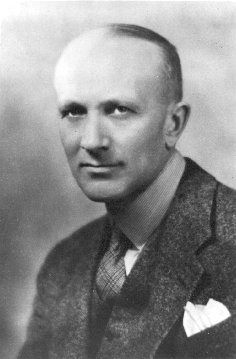
\includegraphics[width=0.8\textwidth]{../resources/illustrations/penfield}
  \caption{Wilder Penfield}
  \end{figure}
\end{minipage}

Peu importe son ou ses origines, le langage est une technologie de l'information primordiale. Il permet un transfert d'informations entre membres d'une société mais aussi, par le bias des traditions orales, un stockage de l'information pendant une durée théoriquement infini. Chez les peuples alettrés une deuxième invention, la structure d'épopée, est souvent utilisé pour faciliter partage et mémorisation des récits sous form de poésies rythmés \cite{havelock-preface-plato}. Notons d'ailleurs que la poésie est toujours utilisé aujourd'hui comme exercise de mémorisation (à l'école) et moyen mnémotechnique (dans la publicité).

\begin{figure}[H]
\centering

\includegraphics[width=0.5\textwidth]{../resources/illustrations/daucy}
\caption{\og{}Sitôt cueilli, sitôt D'Aucy~!\fg{}}
\end{figure}


\chapter{L'écriture~: mémoire externe}
Si le langage peut être vu comme un instinct plutôt qu'une technologie, ce n'est pas le cas de l'écriture. L'écriture idéographique n'est apparu, il y environ 5000 ans, chez un nombre limité de civilisations. L'écriture alphabétique d'ailleurs semble n'être apparu qu'une seule fois, chez les Cananéens, il y a 3700 ans\cite{linguistics-pinker}. Toute autre écriture alphabétique se serait donc dérivé de celle-ci.
%\gls{Écriture alphabétique~: écriture où chaque symbole correspond à un son vocal.}

En tout cas l'invention de l'écriture est une véritable épiphanie informatique. Elle permet à un support mort de stoquer un ensemble de données codés sous forme de symboles, donc de repousser d'avantage la frontière de l'espace et du temps.
Cette avancé rend assez redondants les techniques de mémorisation lyriques mentionnées ci-dessus. La réaction de ceux qui se sont investies dedans est donc peu surprenant~:

\begin{coolquote}[Platon\cite{plato-phaedrus}]
Elle ne peut produire dans les âmes, en effet, que l’oubli de ce qu’elles  savent en leur faisant négliger la mémoire. Parce qu’ils auront foi dans  l’écriture, c’est par le dehors, par des empreintes étrangères, et non plus du dedans et du fond d’eux-mêmes, que les hommes chercheront à se ressouvenir. Tu as trouvé le moyen, non point d’enrichir la mémoire, mais de conserver les souvenirs qu’elle a. Tu donnes à tes disciples la présomption qu’ils ont la science, non la science elle-même. Quand ils auront, en effet, beaucoup appris sans maître, ils s’imagineront devenus très savants, et ils ne seront pour la plupart que des ignorants de commerce incommode, des savants imaginaires au lieu de vrais savants.
\end{coolquote}

Cette critique fait à travers un dialogue entre Socrates et Phaedrus, suggère que l'écriture, en plus de nuire à la mémoire, limite son lecteur à ce que la taxonomie de Bloom\cite{tax-bloom} appelerait \og{}connaître\fg{} à la différence de \og{}comprendre\fg{}, \og{}appliquer\fg{} et cetera. Pour Platon une conaissance ne peut être transféré correctement sans être assimilé, or le papier, si bien soit-il capable de stoquer des propos, est incapable de les comprendre ou de les défendre. 

Il ne faut pas oublier, cependant, que Platon était un professeur dont la pédagogie se repossait sur le dialogue et non la lecture. Il n'est donc pas un interlocuteur très objective. Notons également avec ironie que si nous connaissons Platon c'est grâce à l'écriture, et si nous confondons Socrates avec lui c'est que ce dernier n'a laissé aucune trace écrite.

Celà étant, les critiques de Platon sont d'autant plus pertinents aujourd'hui~: la consultation d'informations est maintenant tellement facile que la mémorisation semble suranné, mais il y une distinction importante à faire entre éfleurer un propos et l'assimiler. Quand nous nous approprions vraiment d'un propos c'est bien plus qu'une copie supplémentaire redondant.

\chapter{L'imprimerie~: reproduction des données}


\chapter{L'horloge maritime~: calcul automatique}
Nous pourrions remplir un rapport tout entier s'il était question d'énumérer les apports de l'outil logico-mathématique, donc nous nous limiterons à l'exemple pertinente des tables de logarithmes. Les logarithmes de Napier, introduits en 1614 dans son oeuvre \og{}Mirifici Logarithmorum Canonis Descriptio\fg{}, furent un outil abstrait visant à simplifier des calculs complexes. Les tables de logarithmes sont très vite devenus indispensables pour tout mathématicien, ingénieur, navigateur ou scientifique.

\begin{coolquote}[Pierre-Simon Laplace\cite{history-of-astronomy}]
[Les logarithmes sont] un artifice admirable qui, en réduisant à quelques jours un travail de plusieurs mois, double la durée de vie de l'astronome, et lui épargne les erreurs et le dégoût : plaies inséparables des longs calculs.
\end{coolquote}

L'utilisation des logarithmes se repose sur des tables de précalcule tels l'\oe{}uvre de 1617 d'Henri Briggs. Muni d'une telle table la multiplication de deux nombre, par exemple, devient triviale~:

\begin{eqnarray}
                    &x            &= 2.16\times{8.13}              \nonumber \\
        \implies{}  &\log{x}      &= \log{2.16}+\log{8.13}         \nonumber \\
                    &             &= 0.3344548 + 0.9100905         \nonumber \\
                    &             &= 1.2445443                     \nonumber \\
        \implies{}  &x            &\approx{17.56}                   \nonumber \\
\end{eqnarray}

La table nous donne directement $\log{2.16}$ et $\log{8.13}$, et nous pouvoir également lire que le logarithme le plus proche est $log{17.56} = 1.2445245$. Nous en déduisons donc en quelques instants $2.16\times{8.13} \approx{17.56}$, ce qui n'est pas loin de de la vraie valeur $2.16\times{8.13}={17.5608}$.

Laplace parle de l'astronome, car il s'agit de l'époque des grandes découvertes~: pour naviger on ne peut s'en passer des almanachs astrales et des algorithmes de navigation astronomique qui se reposaient dessus. Cependant si la latitude peut se calculer grace à l'hauteur perçu du soleil, la longitude est déterminé à partir de la conaissance de l'heure exacte en un endroit précis~: $4$ minutes de décalage correspond à une différence de longitude de $1^{\circ}$.  

En 1714, alors que la flotte Anglaise vient de perdre 1,400 hommes et 4 navire suite à un mauvais calcul de position, le parlement offre un prix de \pounds{20,000} à celui qui saura déterminer, avec une erreur maximum de 56 km, la longitude d'un navire en mer\cite{longitude}. Entre en jeu le charpentier John Harrison, qui construit 1736 la première horloge capable de fonctionner en voyage maritime, suivi d'autres toujours plus compactes et toujours plus précises. Cette invention fut cependant rejeté par l'orthodoxie académique de l'époque, qui voulaient surtout une solution algorithmique tel la méthode des distances lunaires, introduite en Angleterre en 1674 et perfectionnée par Nevil Maskelyne en 1767\cite{history-longitude}. Harrison aura besoin d'attendre 1773 pour recevoir une prime réduite de \pounds{8,750}, et ne sera pas officiellement reconnu comme gagnant.

Pourqui ce rejet? Il s'agit d'un Homme ayant conçu un \og{}oracle\fg{} capable de résoudre le problème pour lui et non pas, distinction importante, une méthode lui permettant de le résoudre lui-même. L'informaticien devient alors prêtre d'un Dieu-machine plutôt que mathématicien-philosophe~: proposition controverse. Ce débat, entre ingénierie et science, trouve son écho aujourd'hui autour de l'apprentissage automatique~: nous pouvons concevoir des machines capable de reconaître des visages, sans comprendre pour autant comment fonctionne cette reconaissance. 

Notons également que de nos jours les algorithmes de calcul à base de tables logarithmiques ne sont même pas introduites à l'école~: la popularisation de calculatrices électroniques aux année 1970 leur ont rendus désuets, de même que l'écriture rend inutile l'épopée. Si des machines à calculer tels le Boulier existent depuis environ 4000 ans, ceux-ci ne sont véritablement que des supports mémoires~: c'est l'étudiant qui applique l'algorithme permettant de calculer le résultat désiré. 

Nous pouvions nous dire que le calcul mentale n'a peu d'importance maintenant que les machines à calcul sont omniprésent, mais la foi en une machine n'est pas moins dangereux que la foi en générale, s'il est sans mesure. 


\chapter{Les technologies du \og{}Broadcast\fg{}~: presse, radio, télévision, internet, \ldots}


%\subsection{Les tournant majeur des technologies de l'information}
//@? Comment introduire la notion de document ?

Les technologies de l'information n'ont eu de cesse de repousser les limites de
la propagation de l'information, 

Avec l'arrivée de l'imprimante, l'Homme est désormais capable de copier
rapidement une information pour la \emph{diffuser}. (Apparition d'une sorte
de broadcast)

Avec le téléphone, l'Homme peut désormais échanger \emph{en tant réelle} une 
information avec une autre personne \og{}~n'importe où~\fg{} dans le monde.

La télévision permet non seulement de faire de même avec des images, mais elle,
ou plutôt son usage, permet bien plus. Elle permet de préformater un document pour ensuite le
diffuser et éventuellement le rediffuser à l'attention d'un public nombreux et
hétérogène tel que l'on peut le faire avec un livre.

Puis vint Internet \og{}~International Network~\fg{}, en vrac: n'importe qui
peut diffuser un document pour un coup très faible, une quantité astronomique
de documents accessibles, Internet se présente comme un méta-outil et offre de
nombreux outils de communication (Mail, Forum, chat, VoIP, conférence, etc...)

\section{en vrac}



Depuis les années 90: internet, outil pour tricher?
%--BROKEN \url{http://www.apsq.org/sautquantique/doss/d-tricherie.html/}

\ldots

\chapter{\ldots dans la société}

La notion de nation est-elle pertinente dans un monde connecté par
internet~?

"The Big Switch: Rewiring the World from Edison to Google" 
 \url{http://www.nicholasgcarr.com/bigswitch/}
 
\begin{coolquote}[Mark Zuckerberg\cite{zuckerberg-privacy-guardian}]
"People have really gotten comfortable not only sharing more information and different kinds, but more openly and with more people," he said. "That social norm is just something that has evolved over time."
\end{coolquote}

Nous perdons notre confidentialité de l'intime. Pour Google, Facebook, etc, 
ce n'est pas un problème: ceux qui n'ont rien à cacher n'ont pas à se soucier. Nous
pouvons cependant noter qu'ils ont intérêt à penser ainsi [j'arrive pas à 
trouver l'article qui en parle]. Le voyeurisme de la télé-réalité montre 
que ce phénomène est de Zeitgeist (esprit de l'époque): nous nous soucions 
moins, par exemple, de qui nous entend parler lors de nos
conversations depuis un téléphone portable.

Les réseaux sociaux permettent un exhibitionnisme, et ceci conduit au 
narcissisme:
http://www.guardian.co.uk/technology/2012/mar/17/facebook-dark-side-study-aggressive-narcissism 
[WHY U NO GIVE ME LINK TO ORIGINAL ARTICLE!]

"The Spy in the Coffee Machine: The End of Privacy As We Know It"
 \url{http://eprints.soton.ac.uk/265683/}

En Février 2010 Eben Moglen lance la notion de "Freedom Box" pour faire face à
la centralisation progressive du web. C'est d'ailleurs sa présentation qui fut
l'amorce du projet Diaspora, visant à créer une plateforme sociale décentralisé 
respectant la confidentialité de ses usagers. 

\section{\ldots par les individus}



\clearemptydoublepage
% !TEX encoding = UTF-8 Unicode
% !TEX root = rapport.tex

\chapter{Les conséquences d'évolutions divergentes}
Du constat de la dichotomie dans l'intégration de la technologie par la société et par l'éducation, émerge un questionnement : quelles sont les conséquences de ce décalage pour les individus ?



\section{Décrochages et échecs scolaires}

\subsection{Manque de pertinences de évaluation}
\subsection{Classification des élèves par tranche d'âge et non par besoins / capacités}
\subsection{Triche <-> coopération}
\subsection{Hyperactivité chez les gamins qui ont juste besoin d'autre chose}
% auto-formation

\section{La formation des étudiants en inadéquation avec les besoins de la société / de l'industrie}


\section{Les retombées imprévues de l'utilisation des technologies de la communication}

\subsection{Piège de Facebook pour les jeunes}


\clearemptydoublepage
% !TEX encoding = UTF-8 Unicode
% !TEX root = rapport.tex

\chapter{Quelles sont les initiatives mises en place pour contrer le phénomène de débilisation des individus par l'informatique}\label{initiatives_actuelles}

\section{Initiatives des pouvoirs publics}

\subsection{Mesures des pouvoirs publics français}
\subsubsection{Mesures en faveur de la prise en main de l'outil informatique}
\cite{b2i_c2i}
\cite{b2i}
\cite{isn}

\subsubsection{opérations "portables" visant à l'accès du plus grand nombre à l'informatique}
\cite{portables35}
\cite{portables60}
\cite{portables40}

    


\subsection{Mesures des pouvoirs publics internationaux}
Forum mondial sur l’éducation \cite{educ_forum}
Les TIC au service de l’éducation \cite{tics}
Un regard sur la trajectoire de l’informatique éducative au Brésil \cite{peixoto2006regard}
Willem J. PELGRUM, Arian T. SCHIPPER, "Indicators of computer integration in education" \cite{pelgrum1993indicators}



\section{Initiatives des acteurs privés}



\section{Quelles peuvent être les solutions adaptées pour endiguer le phénomène ?}\label{solutions}

Interactions entre professeur et élèves
Révision des programmes
Utilisation des nouvelles technologies au service des interactions
Changements des règles de constitution des classes : pourquoi par tranches d'âge ?
Personnalisation des parcours en fonction des envies des élèves.



\clearemptydoublepage
% !TEX encoding = UTF-8 Unicode
% !TEX root = rapport.tex

\part{Conclusion}\label{conclu}

\chapter*{L'effet dominos}
Nous avons vu lors de la première partie que de tous temps les sociétés ont une certaine réticence aux innovations technologiques. Au niveau du système éducatif et de l'arrivée des ordinateurs personnels, cela a rapidement créé un décalage entre la société et les écoles. Ce décalage occasionne de nombreux troubles, comme la difficulté à l'insertion professionnelle, de nombreux échecs scolaires (distraction des élèves), voir de tragiques évènements comme le suicide de jeunes pris aux piège de la diffusion de contenus intimes via internet (voir seconde partie).

\begin{figure}[H]
  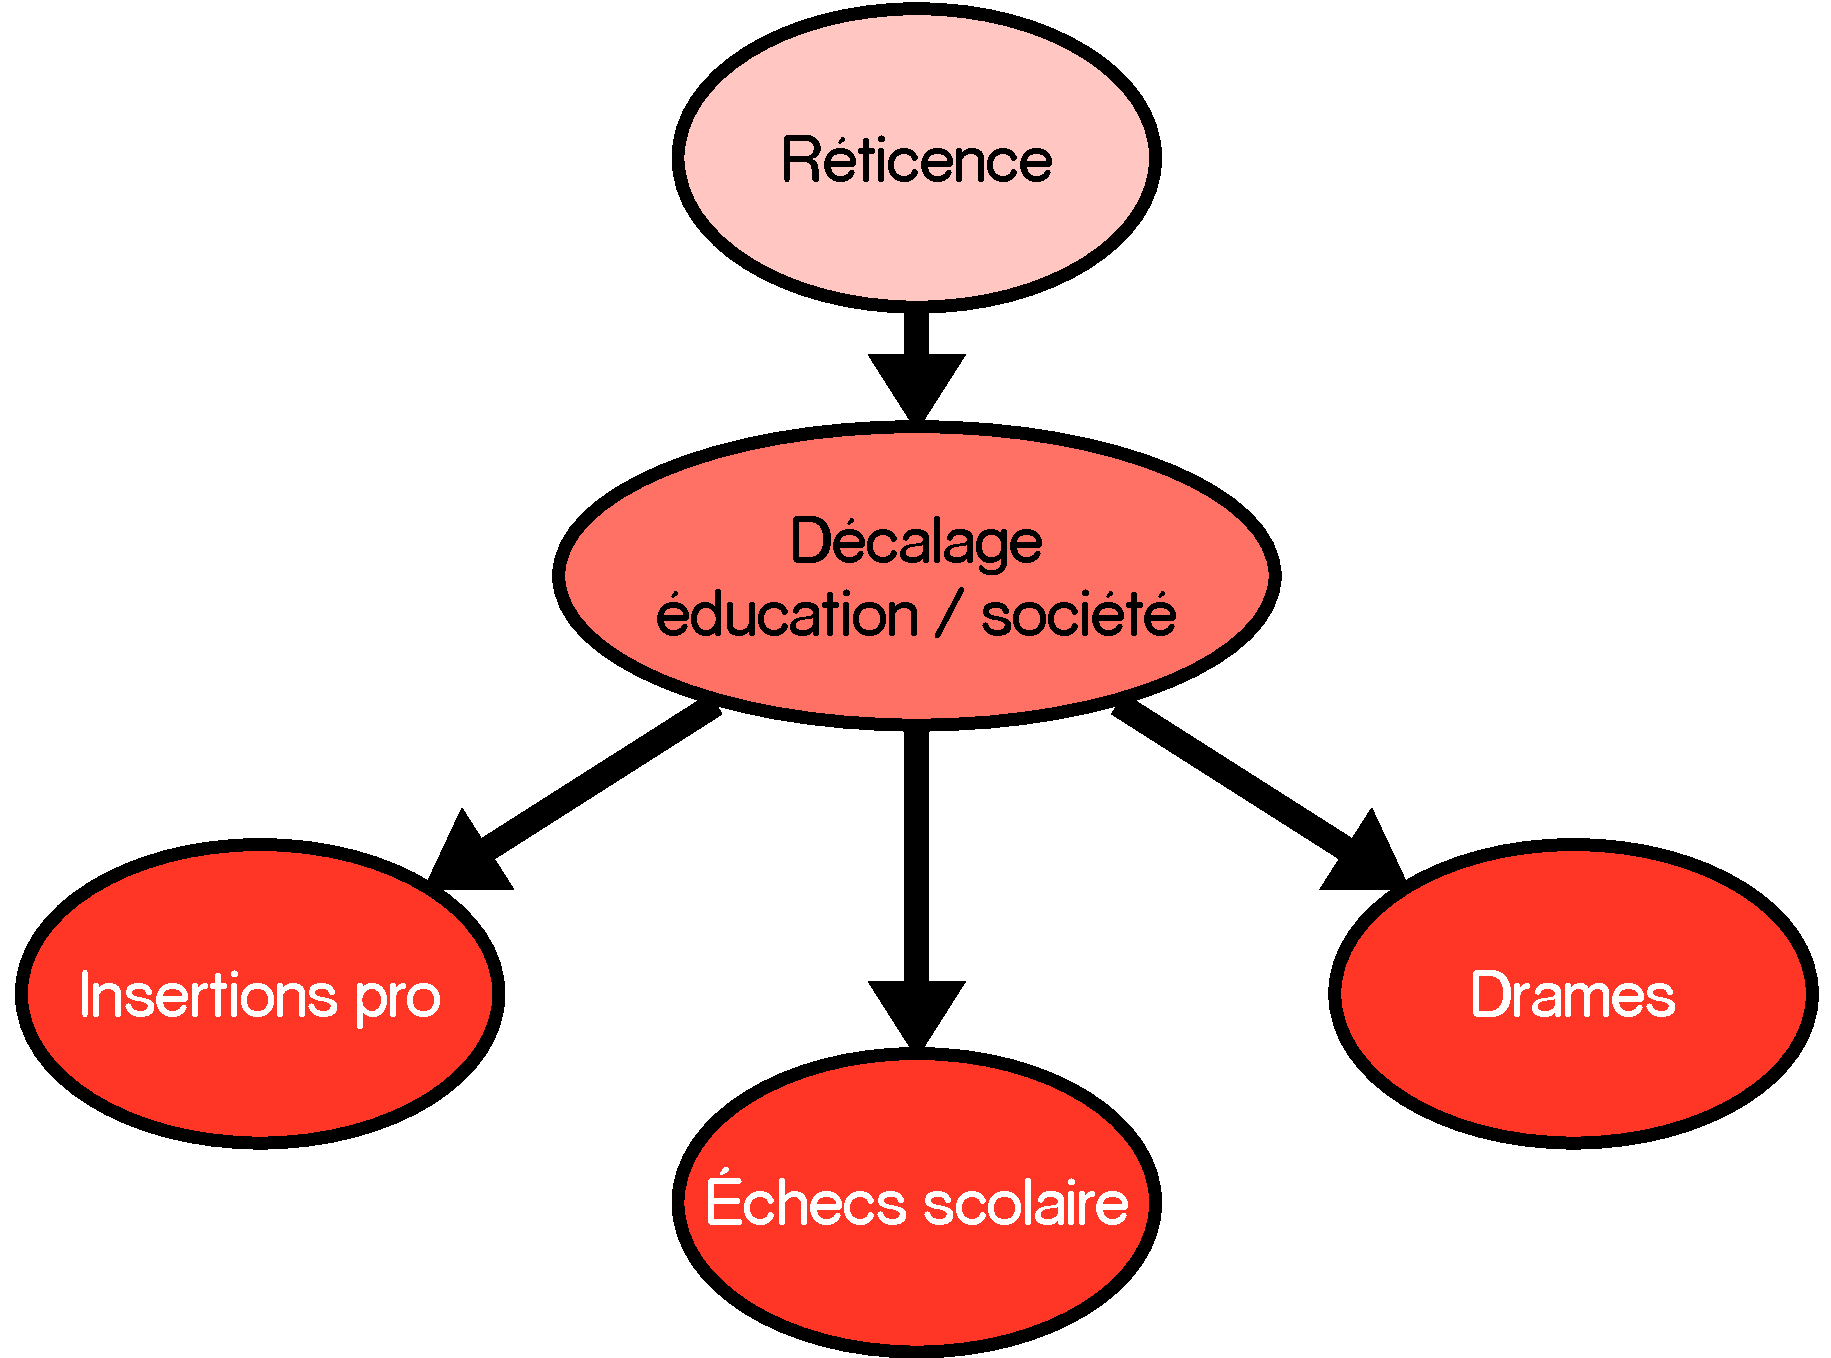
\includegraphics[width=\textwidth]{../resources/illustrations/ccl}
  \caption{Effet dominos causé par la réticence du système éducatif à l'intégration des \gls{ntic}.}
\end{figure}

\chapter*{Concrètement}
Comment pourrions-nous améliorer le système éducatif concrètement ? Nous avons tenu à rappeler quelques points, certainement classés du plus simple au plus complexe à mettre en œuvre.

\begin{description}
  \item[Projets vs. Problèmes] : un élève ne sera naturellement pas impliqué dans la résolution d'un problème dont la correction est donnée 15 minutes plus tard. Ici nous proposons de regrouper et d'inclure ces problèmes dans des projets globaux, effectués en groupes pour favoriser les interactions, et cela sur plusieurs jours (de deux jours à une semaine).
  \item[Multi-niveaux] : bien que le découpage des classes par âge n'ait pas vraiment de sens face à un découpage par centres d'intérêts ou de compétences, nous comprenons bien difficulté de gestion administrative. C'est pourquoi nous proposons, tout en conservant cette répartition par âge, de ne plus voir les différents niveaux comme des frontières, afin de pouvoir organiser des projet mixtes multi-niveaux. Cela permettrait un enrichissement mutuel, notamment les plus jeunes apportent une vision nouvelle sur certains problèmes, et les plus âgés auront tendance à prendre le rôle d'encadrant et d'enseignant.
  \item[Multi-disciplinaires] : beaucoup de sujets regroupent en fait de nombreux domaines. L'idée de briser les frontières entre les disciplines permettrait la réalisation de projets extrêmement intéressants au travers de sujets transversaux en mêlant plusieurs enseignements voir sections ou cursus universitaires.
  \item[Concret avant Abstrait] : idée essentielle et facile à appliquer qui découle directement de la philosophie du contructionnisme : toujours confronter l'élève à la problématique avant de lui enseigner des problèmes concrets.
  \item[Investissement sur l'avenir] : le constat est simple, le système éducatif devrait faire comme le font les grandes entreprises en investissant sur l'avenir. Il serait certainement plus raisonnable d'effectuer des recherches pour développer de nouvelles méthodes d'éducation plutôt que de renouveler les parcs informatiques.
\end{description}

\chapter*{Vers les neurosciences\ldots}
Avant de clôturer ce rapport, nous souhaitons souligner le fait que d'autre méthodes d'apprentissages existent, notamment basées sur les neurosciences. En effet de réels progrès ont eu lieu dans ce domaine ces dix dernières années, ce qui a permis, grâces aux connaissances acquises sur le fonctionnement du cerveau, de mettre en place des exercices adaptés \cite{neurosup}. Particulièrement, nous savons que la réalisation d'un résumé en fin de cours, de préférence sous la forme d'une carte mentale favorise grandement la mémorisation des leçons.

\begin{figure}[H]
  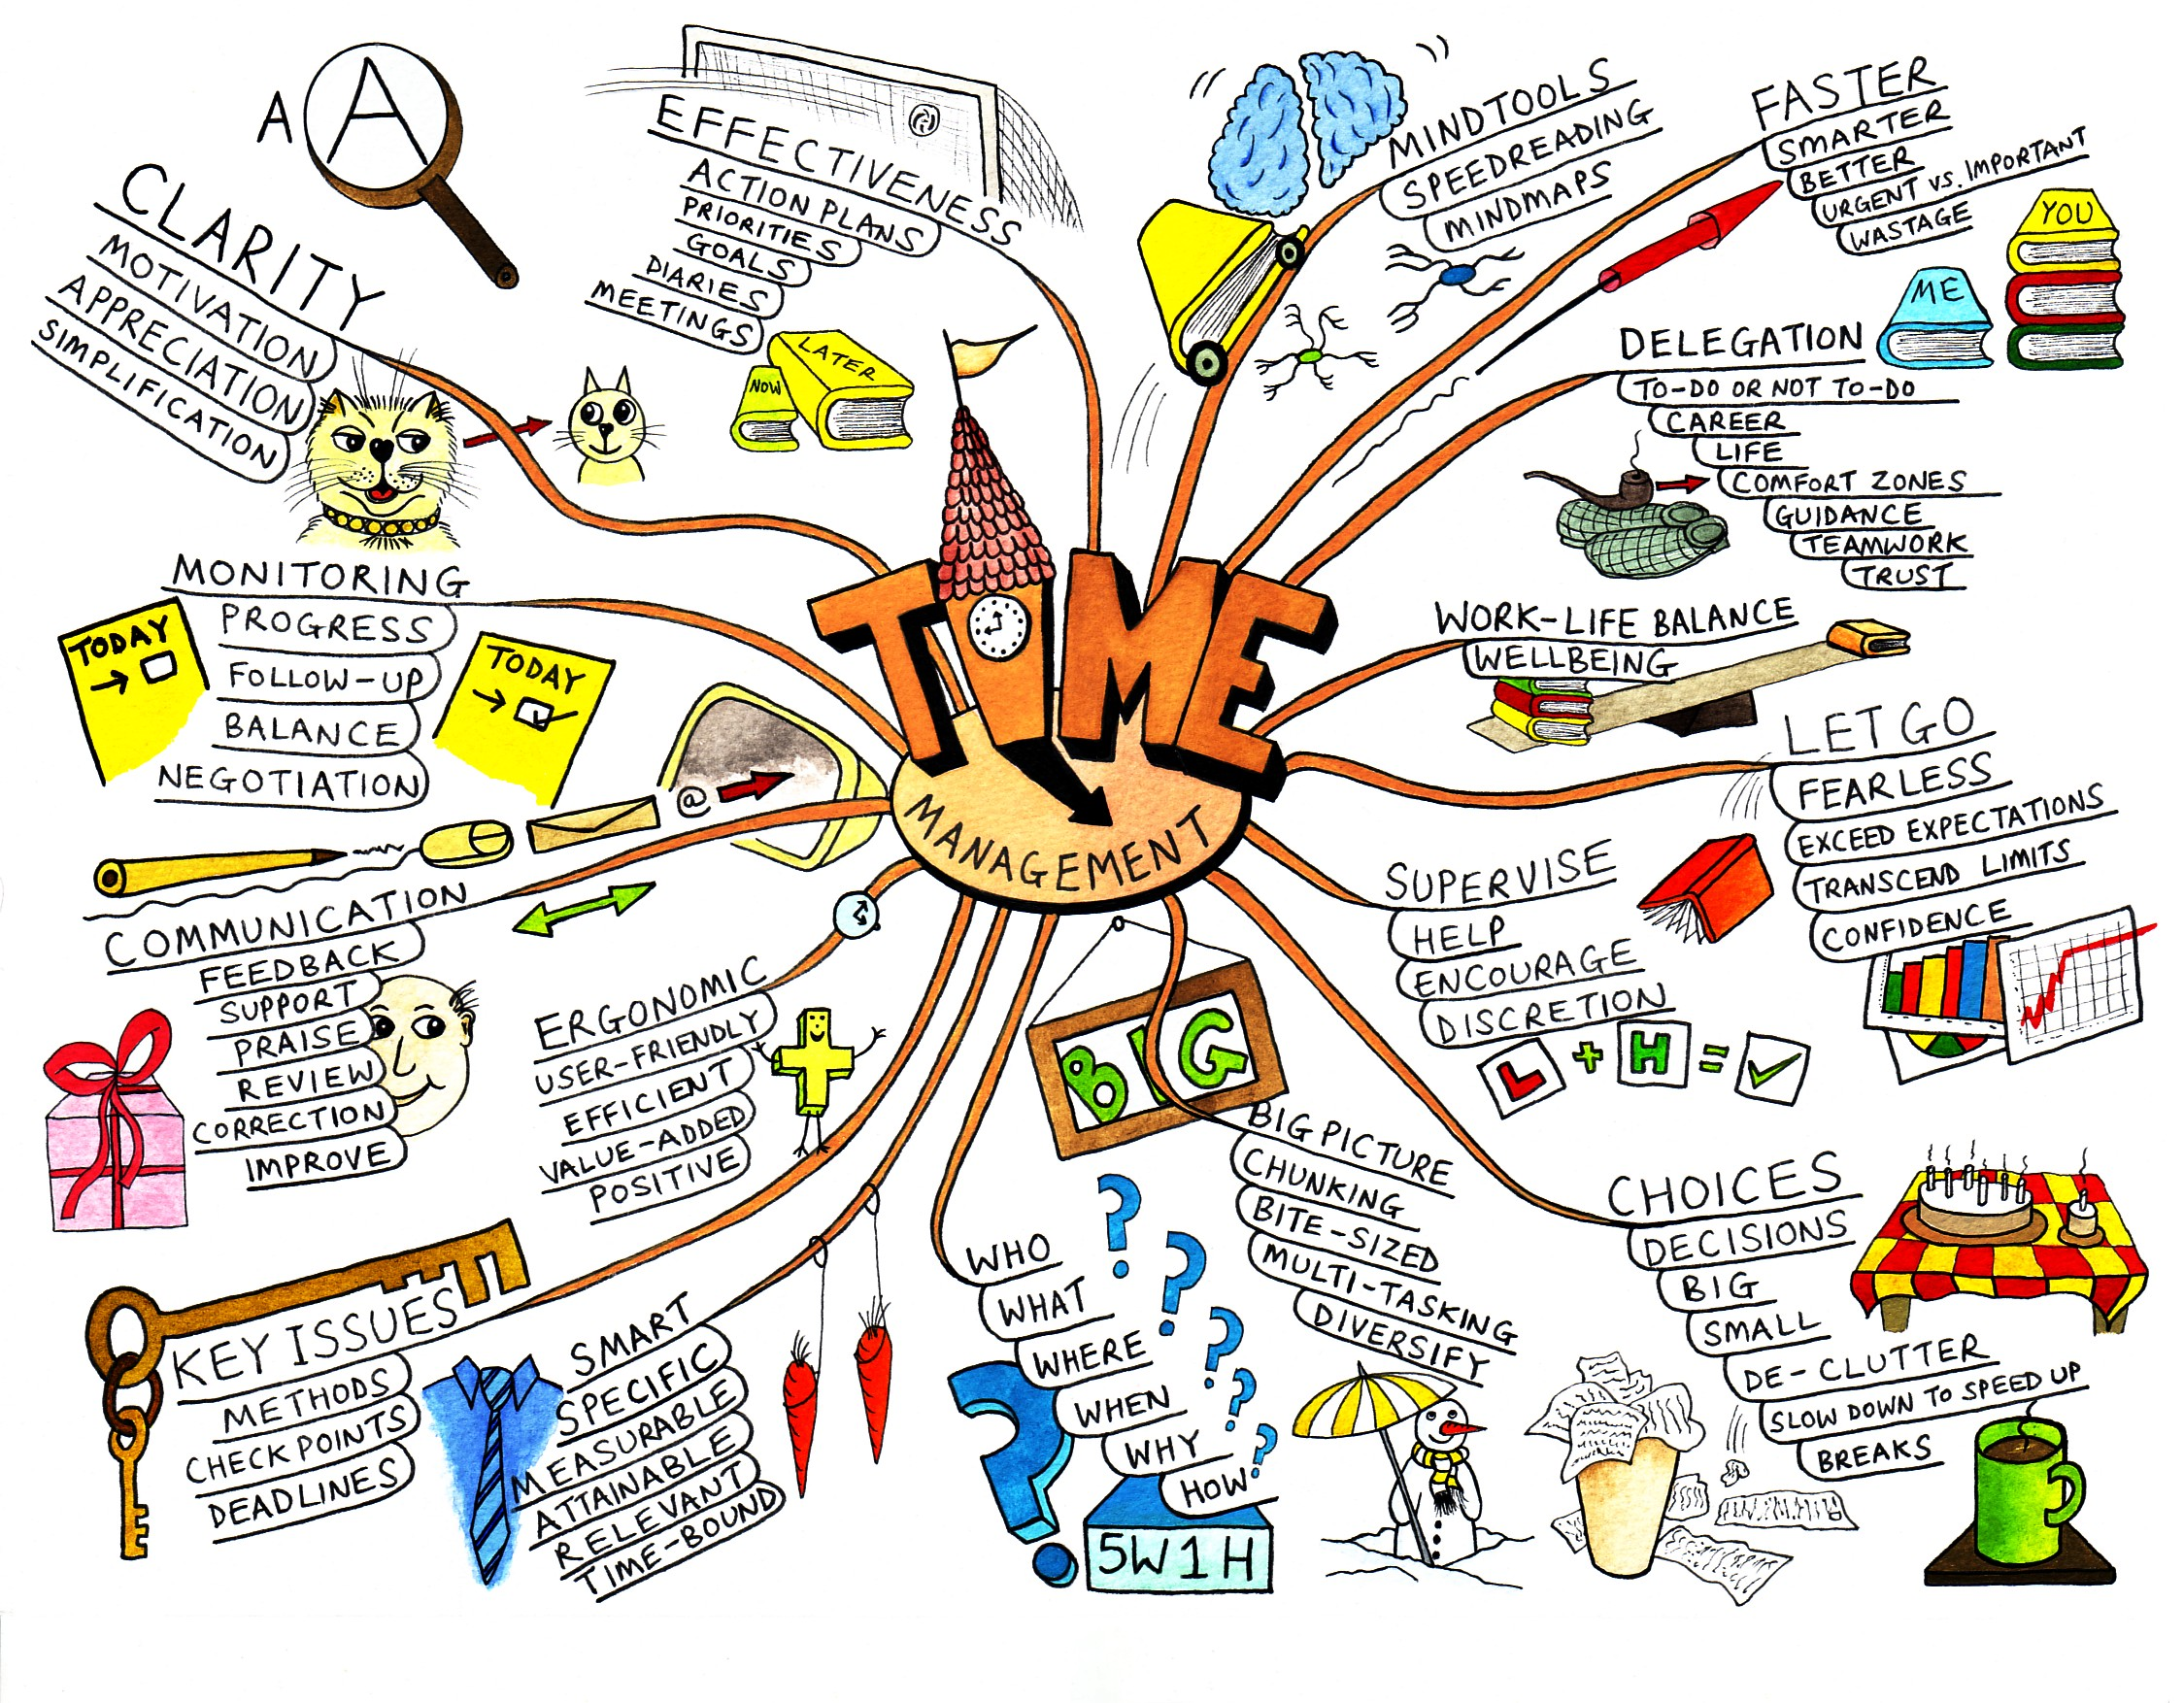
\includegraphics[width=\textwidth]{../resources/illustrations/mindmap}
  \caption{Exemple de carte mentale.}
\end{figure}

Ajoutons tout de même que les méthodes d'apprentissage qui résultent des résultats obtenus dans le domaine des neurosciences n'entrent pas forcément en opposition avec le constructionnisme. Nous somme convaincu par le fait que rester ouvert aux différentes sphères de la recherche permettra de développer de meilleurs approches concernant l'apprentissage et le système éducatif en général.
\clearemptydoublepage

\pagebreak

\addcontentsline{toc}{chapter}{Bibliographie}
\bibliographystyle{plain}
\bibliography{../Bib}
\pagebreak
 
\addcontentsline{toc}{chapter}{Glossaire}
\printglossaries
\pagebreak
 
\addcontentsline{toc}{chapter}{Table des figures}
\listoffigures

\vfill
{\raggedleft Réalisé avec \LaTeX{} \par}

\end{document}

